\chapter{Nombres rationnels}

\section{Rappels et vocabulaire}
%La division de 2 par 5 peut être notée sous forme d'une fraction: $\frac{2}{5}$.
Toute fraction représente une division qu'on n'effectue pas:
$$ \dfrac{5}{2} = 5:2. $$
Comme il n'est pas possible de diviser par 0, le D (=dénominateur) ne peut pas être 0.
\\
\id{Vocabulaire numérateur, dénominateur opschreiwen am Beispill uewendriwwer}

\begin{enumerate}[label=$\triangleright$]
	\item Diviser le N et le D par un même nombre est appelé \og\emph{simplifier}\fg{}:
				$$ \dfrac{10}{15} = \dfrac{2 \cdot 5}{3 \cdot 5} = \dfrac{2}{3} $$
  \item On ne peut pas simplifier si le N ou le D sont une somme, une différence ou une division. Dans ce cas, on doit d'abord effectuer:
    		$$ \frac{6+2}{4} = \frac{8}{4}=2 $$
	\item Une fraction est appelée \og\emph{irréductible}\fg{} si les N et le D sont des entiers et si la fraction ne peut pas être simplifiée.
	\item Multiplier le N et le D par un même nombre est appelé \og\emph{amplifier}\fg{}:
				$$ \dfrac{1}{2,7} = \dfrac{10}{27} $$
	\item Chaque entier peut être écrit sous forme fractionnaire:
				$$ 3=\frac{3}{1};\quad 5 = \dfrac{5}{1};\quad 13 = \dfrac{13}{1} $$
	\item Mais:
				$$ 1=\frac{1}{1} = \dfrac{2}{2} = \dfrac{3}{3} = ... $$
\end{enumerate}

\rem{Le trait d'une fraction s'écrit toujours à la même hauteur que le signe de l'égalité!
\id{Laisser vérifier (et corriger) les élèves dans leur propre cahier.}}

\rem{Une fraction comportant des nombres décimaux n'est pas appelée \og{}fraction\fg{}, mais \og{}écriture fractionnaire\fg{}.
}

Mathematic:
\begin{center}
	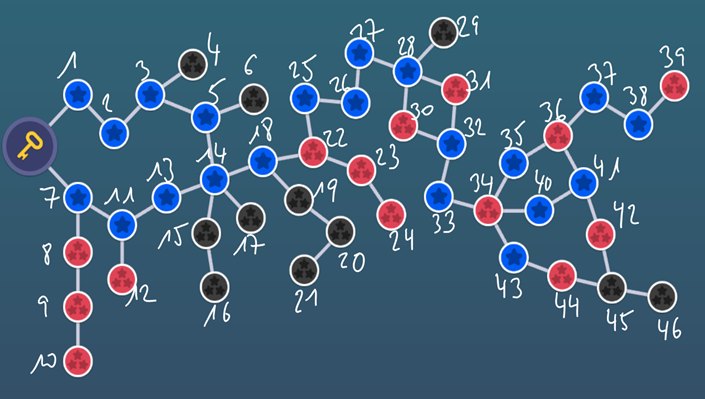
\includegraphics[width=8cm]{pictures/mathematic_nombres_en_ecriture_fractionnaire}
\end{center}
Items à faire: (la majorité représente un rappel de la 7e et ne traite que les nombre positifs.)
\begin{enumerate}[label=+]
	\item 8, 9, 10: rappels fraction <-> surface coloriée/surface totale.
	\item 12: placer des fractions sur une demi-droite.
	\item[-] 15, 16: revient à déterminer le pgcd de deux (ou 3) nombres. (16 un peu difficile pour une base.)
	\item 17: repérer une surface qui représente la fraction (proportion) donnée.
	\item 19, 20, 21: domino et triomino.
	\item 22, 23, 24: ordonner des fractions.
	\item[-] 29: laisser faire un peu plus tard (égalité de fractions avec calculs).
	\item 30, 31: addition et soustraction de fractions.
	\item 34, 36: multiplication et priorité.
	\item[-] 39: chercher l'intrus avec fractions, nombres et figures.
	\item 42: division, est traité aussi dans ce cours.
	\item 44: multiplication de plusieurs fractions.
	\item[-] 45, 46: jeux où on doit relier les calculs avec fractions avec leur résultat.
\end{enumerate}

\id{Fir des Kapitel sinn ca. 3-4 Wochen virgesinn.
Vu que den Inhalt vum mathematic e Rappell ass, kéint een si am Ufank vum Kapitel an de Stonnen e bësse schaffe loossen a parallel ëmmer e bëssen als Hausaufgab.
Fir dat ganzt Kapitel am Mathematic serieux ze maachen, brauch een mindestens 6 Stonnen schätzen ech, dowéinst wier et evt. besser déi schwaarz eweg ze loossen an als Bonus ze ginn.
\\
Verschidde Beispiller aus den Exercicen sinn fir den Niveau de base villäicht ze schwéier... à voir.
}


\section{Fractions négatives}
$\dfrac{3}{5} > \dfrac{1}{5}$ mais $-\dfrac{3}{5} < -\dfrac{1}{5}$.
\\
\id{Placer sur l'axe des abscisses.}

%De même: $\frac{1}{2} > \frac{1}{3}$ mais $-\frac{1}{2} < -\frac{1}{3}$.

\rem{Il est plus facile de comparer les fractions si on réfléchit si elles sont comprises entre 0 et -1 ou inférieures à -1.
}

\renewcommand{\arraystretch}{1.5}
$$\begin{array}{ccp{.5cm}l}
	\textbf{Division} & \textbf{Signe du résultat} && \textbf{Écriture fractionnaire} \\
	(-1):(+2) & \red négatif && \dfrac{-1}{2} = {\red -}\dfrac{1}{2} \\
	(+1):(-2) & \red négatif && \dfrac{1}{-2}= {\red -}\dfrac{1}{2} \\
	(-1):(-2) & \green positif  && \dfrac{-1}{-2}={\green +}\dfrac{1}{2} = \dfrac{1}{2}
\end{array}$$
\renewcommand{\arraystretch}{1.2}

Finalement:
$$ \boxed{\frac{-1}{2}=\frac{1}{-2} =-\frac{1}{2}} \quad \text{et} \quad \boxed{\frac{-3}{-5}=+\frac{3}{5}} $$
et en général:
\prop{Quels que soient les nombres $a$ et $b$ avec $b\overset{!}{\neq}0$:
$$ \dfrac{-a}{-b}=\dfrac{a}{b}  \qquad\text{et}\qquad  \dfrac{-a}{b}=\dfrac{a}{-b}=-\dfrac{a}{b} $$
}

\rem{Il faut mettre des parenthèses, car le signe se rapporte à tous les termes du numérateur:
$$ -\dfrac{2+7}{3} = \dfrac{-(2+7)}{3}. $$
}


%Ex. 38,41,42,44,45,47 p.57 (T4) \datei{Bicher/T4/T4_p.057.jpg} \\
%Ex. 125 p.63 \datei{Bicher/T4/T4_p.063.jpg}



\subsection{Addition et soustraction de fractions}
\addexo{Effectue les calculs suivants et donne le résultat sous forme d'une fraction irréductible.
\begin{multicols}{2}
\begin{enumerate}[itemsep=.25cm]
  \item $ \dfrac{1}{2}+\dfrac{1}{4} $
  \item $ \dfrac{1}{3}-\dfrac{1}{4} $
  \item $ 0,3 +0,\overline{3} $
  \item $ 0,\overline{6}-0,6 $
  \item $ \dfrac{3}{4} {\green +} \dfrac{{\red -}2}{5}$ 
  \item $ \dfrac{5}{20} + \dfrac{3}{15} +\dfrac{15}{25} $
\end{enumerate}
\end{multicols}
}{
\begin{enumerate}[label=\alph*)]
  \item $ \frac{1}{2}+\frac{1}{4} = $
  \item $ \frac{1}{3}-\frac{1}{4}= $
  \item $ \frac{3}{4} {\green +} \frac{{\red -}2}{5} =  \frac{15}{20} {\green +} \frac{{\red -}8}{20} = \frac{15{\green +}({\red -}20)}{7} = \frac{-5}{20} = -\frac{1}{4} $ 
  \item $ \frac{5}{20} + \frac{3}{15} +\frac{15}{25}= $
\end{enumerate}
}

\ret{Pour faciliter un calcul avec fractions, on effectue dans ordre suivant:
\begin{enumerate}
	\item Écrire les nombres décimaux sous forme de fractions (avec entiers).
	\item Simplifier les fractions autant que possible.
	\item Déterminer les DC pour les additions et les soustractions.
	\item Effectuer les opérations tout en respectant les règles de priorités: \\
				parenthèses $\rightarrow$ multiplications $\rightarrow$ additions/soustractions.
	\item Simplifier le résultat final afin d'obtenir une fraction \emph{irréductible}.
\end{enumerate}
}

\addexo{Calcule.
\begin{multicols}{2}
\begin{enumerate}[itemsep=.25cm]
  \item $ \dfrac{3}{4}+\dfrac{5}{6}-\dfrac{7}{12} $
  \item $ \dfrac{46}{16}-\dfrac{5}{3}-\dfrac{4}{12} $
  \item $ \dfrac{3}{2}+\dfrac{8}{12}-\dfrac{16}{20} $
  \item $ \dfrac{11}{12}-\dfrac{15}{20}+\dfrac{14}{21} $
  \item $ \dfrac{2}{3}-\dfrac{3}{4}+\dfrac{5}{2} $
  \item $ \dfrac{30}{54}-\dfrac{66}{121}+\dfrac{6}{9} $
\end{enumerate}
\end{multicols}
}{-}

\addexo{Calcule.
\begin{multicols}{2}
\begin{enumerate}[itemsep=.25cm]
  \item $ \dfrac{3}{4}-\dfrac{1}{6}-\dfrac{1}{9} $
  \item $ \dfrac{10}{15}+\dfrac{15}{12}-\dfrac{20}{18} $
  \item $ \dfrac{3}{4}+\dfrac{7}{8}-\dfrac{4}{3} $
  \item $ \dfrac{18}{20}-\dfrac{8}{60}+\dfrac{21}{35} $
  \item $ \dfrac{98}{100}-\dfrac{196}{200} $
  \item $ 1-\dfrac{8}{12}+\dfrac{18}{15} $
\end{enumerate}
\end{multicols}
}{-}

\addexo{Calcule.
\begin{multicols}{2}
\begin{enumerate}[itemsep=.25cm]
  \item $ \dfrac{3}{8}+\dfrac{35}{14} $
  \item $ \dfrac{13}{3}-\dfrac{4}{9} $
  \item $ \dfrac{13}{3}-\dfrac{4}{9} $
  \item $ 0,625+\dfrac{7}{4}+\dfrac{33}{22} $
  \item $ \dfrac{1}{2}+0,25+\dfrac{1}{3}-\dfrac{5}{6} $
  \item $ \dfrac{11}{12}-0,75+\dfrac{10}{15} $
\end{enumerate}
\end{multicols}
}{
\begin{multicols}{2}
\begin{enumerate}
  \item $ \dfrac{23}{8} $
  \item $ \dfrac{35}{9} $
  \item $ \dfrac{35}{9} $
  \item $ \dfrac{31}{8} $
  \item $ \dfrac{1}{4} $
  \item $ \dfrac{5}{6} $
\end{enumerate}
\end{multicols}
}

\addexo{Calcule.
\begin{enumerate}[itemsep=.25cm]
  \item $ \dfrac{14}{21}-\left( \dfrac{15}{20}+2,5-\dfrac{5}{12} \right) $
  \item $ \dfrac{17}{12}-\dfrac{5^2}{18} $
  \item $ \dfrac{10}{15}-\dfrac{15}{12}-\dfrac{20}{18} $
  \item $ -\dfrac{11}{21}-\dfrac{18}{35} $
  \item $ -\dfrac{66}{39}+\dfrac{4^3}{26}-\left(\dfrac{72}{52}-\dfrac{30}{65}\right) $
  \item $ \dfrac{35}{10}-\left( \dfrac{39}{78}-\dfrac{12}{56} \right) $
\end{enumerate}
}{
\begin{enumerate}
  \item $ -\dfrac{13}{6} $
  \item $ \dfrac{1}{36} $
  \item $ -\dfrac{61}{36} $
  \item $ -\dfrac{109}{105} $
  \item $ -\dfrac{2}{13} $
  \item $ \dfrac{45}{14} $
\end{enumerate}
}

\addexo{Calcule.
\begin{enumerate}[itemsep=.25cm]
  \item $ -\dfrac{21}{56}+\dfrac{32}{88}-\dfrac{17}{34} $
  \item $ \dfrac{9}{14}-\dfrac{3}{21} $
  \item $ -0,6-\dfrac{4}{7}-\dfrac{-2}{70} $
  \item $ -\left(\dfrac{36}{96}+\dfrac{20}{55}\right) -\dfrac{22}{44} $
  \item $ -\dfrac{15}{-20-25}-\dfrac{-12}{210}-\left(\dfrac{15}{75}+\dfrac{-9}{-35}\right) $
  \item $ \dfrac{16+2}{16+4}-\dfrac{135-117}{135}+\dfrac{-18}{18+12} $
\end{enumerate}
}{
\begin{enumerate}
  \item $ -\dfrac{45}{88} $
  \item $ \dfrac{1}{2} $
  \item $ -\dfrac{8}{7} $
  \item $ -\dfrac{109}{88} $
  \item $ -\dfrac{1}{15} $
  \item $ \dfrac{1}{6} $
\end{enumerate}
}


%\arrow Ex. 60-65 p.58 (T4) \datei{Bicher/T4/T4_p.058.jpg} \\
%\arrow Ex. 108 p.61 \datei{Bicher/T4/T4_p.061.jpg} \\
%\arrow Ex. 114, 122 p.62 \datei{Bicher/T4/T4_p.062.jpg}



\subsection{Multiplication}
%Un quart de deux tiers:
%\begin{center}
%	\definecolor{qqqqff}{rgb}{0,0,1}
%	\definecolor{qqzzqq}{rgb}{0,0.6,0}
%	\definecolor{cqcqcq}{rgb}{0.75,0.75,0.75}
%	\begin{tikzpicture}[line cap=round,line join=round,>=triangle 45,x=1.0cm,y=1.0cm]
%		\draw [color=cqcqcq,dash pattern=on 1pt off 1pt, xstep=1.0cm,ystep=1.0cm] (0.76,0.75) grid (5.31,4.38);
%		\clip(0.76,0.75) rectangle (5.31,4.38);
%		\fill[color=qqzzqq,fill=qqzzqq,fill opacity=0.1] (1,4) -- (5,4) -- (5,2) -- (1,2) -- cycle;
%		\fill[color=qqqqff,fill=qqqqff,fill opacity=0.1] (1,2) -- (2,2) -- (2,4) -- (1,4) -- cycle;
%		\draw (1,1)-- (5,1);
%		\draw (5,1)-- (5,4);
%		\draw (5,4)-- (1,4);
%		\draw (1,4)-- (1,1);
%		\draw [color=qqzzqq] (1,4)-- (5,4);
%		\draw [color=qqzzqq] (5,4)-- (5,2);
%		\draw [color=qqzzqq] (5,2)-- (1,2);
%		\draw [color=qqzzqq] (1,2)-- (1,4);
%		\draw [color=qqqqff] (1,2)-- (2,2);
%		\draw [color=qqqqff] (2,2)-- (2,4);
%		\draw [color=qqqqff] (2,4)-- (1,4);
%		\draw [color=qqqqff] (1,4)-- (1,2);
%	\end{tikzpicture}
%\end{center}
%
%$$  \dfrac{1}{4} \cdot \dfrac{2}{3} = \dfrac{1}{6} $$
%
%\rem{On n'a pas besoin d'un DC!
%}
%
%%\arrow Ex. 68-77 p.59 (T4) \datei{Bicher/T4/T4_p.059.jpg}
%
%Pour multiplier deux fractions, on:
%\begin{enumerate}
%	\item note d'abord le signe du produit,
%	\item ensuite on simplifie chaque fois un N et un D.
%\end{enumerate}


\addexo{Calcule.
\begin{multicols}{2}
\begin{enumerate}[itemsep=.25cm]
	\item $ -\dfrac{4}{5} \cdot \left( -\dfrac{2}{3} \right) $
	\item $ (-1) \cdot \left( -\dfrac{5}{3} \right) $
	\item $ \dfrac{7}{5} \cdot \left( -\dfrac{3}{4} \right) $
	\item $ \dfrac{31}{5} \cdot \dfrac{-1}{2} $
	\item $ \left( -\dfrac{5}{7} \right)^2 $
	\item $ \dfrac{27}{12} \cdot \left( -\dfrac{1}{3} \right) $
\end{enumerate}
\end{multicols}
}{-}

\addexo{Calcule.
\begin{multicols}{2}
\begin{enumerate}[itemsep=.25cm]
	\item $ -\left(-\dfrac{2}{3} \right)^2 $
	\item $ \dfrac{5}{7} +\left( -\dfrac{6}{7} \right) $
	\item $ -\dfrac{3}{7} \cdot \dfrac{5}{-6} $
	\item $ \left(-\dfrac{1}{2} \right) \cdot \dfrac{3}{4} \cdot \dfrac{-5}{2} $
	\item $ \dfrac{-5}{3} -\dfrac{-(-7)}{-9} $
	\item $ \dfrac{3}{-4} \cdot \left( -\dfrac{1}{2} \right) \cdot \dfrac{-6}{9} $
\end{enumerate}
\end{multicols}
}{-}



\subsection{Division et nombre inverse}
\id{pour 6Gb\,: inverse sans base négative.
}

\id{voir mathematic, item 42.
}

Exemples:
\begin{multicols}{4}
\begin{enumerate}[label=\alph*)]
  \item $ 4 : \ldots = 2$
  \item $ 4 \cdot \ldots = 2 $
  \item $ 6 : \ldots = 1 $
  \item $ 6 \cdot \ldots = 1 $
  \item $ 8 : \ldots = 2 $
  \item $ 8 \cdot \ldots = 2 $
  \item $ 12 : \ldots = 4 $
  \item $ 12 \cdot \ldots = 4 $
\end{enumerate}
\end{multicols}

\prop{Diviser par un nombre non nul $n=\dfrac{1}{n}$ revient à multiplier par son inverse $\dfrac{1}{n}$.
}

On appelle $\frac{1}{4}$ l'inverse de $4$ et $4$ l'inverse de $\dfrac{1}{4}$. \\
De même: $-\dfrac{1}{22}$ est l'inverse de $-22$.

\defn{\emph{Deux nombres} sont \emph{inverses} l'un de l'autre ssi leur produit est égal à 1.
}

Exemples\,: 1; $\frac{1}{3}$; $-3$ $\frac{2}{3}$; $-\frac{3}{7}$.

\rem{$0,25 = \frac{1}{4}$, alors on peut multiplier par 4 au lieu de diviser par 0,25:
$$ 1:0,25 =4, \qquad
5:0,25 = 5  \cdot 4 = 20. $$
}


\addexo{Écris les inverses des nombres suivants.
\begin{multicols}{3}
\begin{enumerate}[itemsep=.25cm]
	\item $\dfrac{3}{2}$
	\item $\dfrac{-3}{4}$
	\item $-\dfrac{7}{6}$
	\item $-2$
	\item $1$
	\item $-1$
\end{enumerate}
\end{multicols}
}{-}

\addexo{Qui a raison? Justifie.

}{-}

\addexo{Calcule.
\begin{multicols}{2}
\begin{enumerate}[itemsep=.25cm]
	\item $ \dfrac{\dfrac{25}{36}}{\dfrac{20}{24}} $
	\item $ -\dfrac{13}{30} : \left(  -\dfrac{1}{11} \right) $
	\item $ \dfrac{-5}{4} : \dfrac{4}{3} $
	\item $ \dfrac{8}{\dfrac{9}{5}} $
	\item $ \dfrac{\dfrac{8}{9}}{5} $
	\item $ \dfrac{3}{5} : (-0,2) $
\end{enumerate}
\end{multicols}
}{-}

\addexo{Calcule.
\begin{multicols}{2}
\begin{enumerate}[itemsep=.25cm]
	\item $ \dfrac{8}{5} -\dfrac{3}{4} $
	\item $ \dfrac{-5}{2} +\dfrac{1}{3} $
	\item $ \dfrac{4}{5} : \dfrac{5}{6} $
	\item $ \dfrac{-4}{3} \cdot \left( -\dfrac{1}{5} \right) $
	\item $ \dfrac{4}{9} +\dfrac{2}{15} $
	\item $ \dfrac{8}{6} :2 $
\end{enumerate}
\end{multicols}
}{-}

\addexo{Calcule.
\begin{multicols}{2}
\begin{enumerate}[itemsep=.25cm]
	\item $ -\dfrac{1}{4} +\dfrac{3}{4} -1,25 $
	\item $ \dfrac{10}{9} -\dfrac{2}{9} +\dfrac{8}{9} $
	\item $ \dfrac{1}{2} -\dfrac{-1}{-4} +\dfrac{3}{-4} $
	\item $ \dfrac{1,5}{2,5} -\dfrac{2+3}{2} -\dfrac{1}{4-1} $
	\item $ \dfrac{3}{8} -\dfrac{5}{2} +\dfrac{1}{6} $
	\item $ \dfrac{10}{3} +1 -\dfrac{1}{2} $
\end{enumerate}
\end{multicols}
}{-}

\addexo{Calcule.
%\begin{multicols}{2}
\begin{enumerate}[itemsep=.25cm]
	\item $ \dfrac{5}{2} +\dfrac{7}{2} :\dfrac{2}{3} $
	\item $ \dfrac{3}{2} \cdot \dfrac{1}{4} +0,375 $
	\item $ \dfrac{5}{2} -\dfrac{1}{2} \cdot 3 $
	\item $ \dfrac{4}{6} -\dfrac{1}{6} \cdot \dfrac{5}{2} $
	\item $ \left( \dfrac{1}{6} -\dfrac{1}{3} \right) \cdot \left( \dfrac{1}{6} +\dfrac{1}{3} \right)  $
	\item $ \left( -\dfrac{1}{5} +\dfrac{3}{5} \right) \cdot \left( \dfrac{1}{4} +\dfrac{5}{2} \right) $
\end{enumerate}
%\end{multicols}
}{-}

\addexo{Calcule.
\begin{multicols}{2}
\begin{enumerate}[itemsep=.25cm]
	\item $ \dfrac{2}{30}+\dfrac{6}{45} \cdot 3 $
	\item $ 3+5 \cdot \dfrac{-42}{49} $
	\item $ 1,25 \cdot \left( \dfrac{15}{10} -\dfrac{2}{16} \right) $
	\item $ \dfrac{7}{4} -\dfrac{3}{4} \cdot \dfrac{40}{45} $
	\item $ \left(1-\dfrac{2}{3} \right) : \left(1+\dfrac{2}{3} \right) $
	\item $ \dfrac{\dfrac{12}{16} +\dfrac{8}{24}}{2 -\dfrac{14}{6}} $
\end{enumerate}
\end{multicols}
}{-}

%\addexo{Calcule.
%\begin{multicols}{2}
%\begin{enumerate}[itemsep=.25cm]
%	\item $  $
%	\item $  $
%	\item $  $
%	\item $  $
%	\item $  $
%	\item $  $
%\end{enumerate}
%\end{multicols}
%}{-}

% Déi nächst Exercicen sinn zum groussen Deel schon oofgetippt.
%\arrow Ex. 78-83 p.59 (T4) \datei{Bicher/T4/T4_p.059.jpg} \\
%\arrow Ex. 84-98 p.60 \datei{Bicher/T4/T4_p.060.jpg}







%%% -------------------------------- EXERCICEN PRINTEN
\clearpage
\begin{exercices}
\foreach \x/\y in \exos
{\exo \x
 \ifnum\value{exo}=5 \columnbreak\fi
 \ifnum\value{exo}=10 \pagebreak\fi
 }
\end{exercices}